%=====================================================================
%  Large-Scale Agricultural Market Data Processing
%  and Real-Time Market Analysis
%
%  Big Data Analytics -- College Project Presentation
%  Compile with:  pdflatex AG-DATA-presentation.tex   (run twice)
%
%  Only standard packages are used (beamer, tikz, booktabs, xcolor),
%  so this compiles on Overleaf or any full TeX Live install.
%=====================================================================
\documentclass[aspectratio=169,12pt]{beamer}

\usepackage[utf8]{inputenc}
\usepackage[T1]{fontenc}
\usepackage{lmodern}
\usepackage{booktabs}
\usepackage{tikz}
\usetikzlibrary{arrows.meta,positioning,shapes.geometric,calc}

%---------------------------------------------------------------
% A simple, consistent colour scheme (agriculture green + amber)
%---------------------------------------------------------------
\definecolor{agriGreen}{RGB}{27,94,32}
\definecolor{agriLight}{RGB}{232,245,233}
\definecolor{agriAmber}{RGB}{230,145,10}
\definecolor{agriGrey}{RGB}{69,90,100}
\definecolor{agriBlue}{RGB}{21,101,192}

\usetheme{default}
\usecolortheme{default}
\setbeamercolor{structure}{fg=agriGreen}
\setbeamercolor{normal text}{fg=agriGrey}
\setbeamercolor{frametitle}{fg=white,bg=agriGreen}
\setbeamercolor{title}{fg=agriGreen}
\setbeamercolor{itemize item}{fg=agriGreen}
\setbeamercolor{itemize subitem}{fg=agriAmber}
\setbeamercolor{block title}{fg=white,bg=agriGreen}
\setbeamercolor{block body}{bg=agriLight}

\setbeamertemplate{navigation symbols}{}
\setbeamertemplate{itemize item}{\textbullet}
\setbeamertemplate{itemize subitem}{--}

% Frame title with comfortable padding and large type
\setbeamertemplate{frametitle}{%
  \nointerlineskip
  \begin{beamercolorbox}[wd=\paperwidth,ht=3.2ex,dp=1.4ex,leftskip=0.8cm]{frametitle}
    \usebeamerfont{frametitle}\insertframetitle
  \end{beamercolorbox}
}
\setbeamerfont{frametitle}{size=\Large,series=\bfseries}
\setbeamerfont{itemize/enumerate body}{size=\large}
\setbeamerfont{itemize/enumerate subbody}{size=\normalsize}

% Slide number in the bottom-right corner
\setbeamertemplate{footline}{%
  \hfill\raisebox{1.2ex}{\color{agriGrey}\small\insertframenumber}\hspace{0.6cm}
}

% Generous spacing between bullets -- keeps slides breathable
\setlength{\parskip}{0.4em}
\newcommand{\bigskipitems}{\setlength{\itemsep}{0.75em}}

% Reusable TikZ box styles for the diagrams
\tikzset{
  flowbox/.style={
    rectangle, rounded corners=3pt, draw=agriGreen, thick,
    fill=agriLight, text=agriGrey, align=center,
    minimum width=3.3cm, minimum height=0.85cm, font=\small\bfseries},
  hilitebox/.style={
    flowbox, fill=agriGreen, text=white, draw=agriGreen},
  ambox/.style={
    flowbox, fill=agriAmber!20, draw=agriAmber},
  arrowline/.style={-{Stealth[length=2.5mm]}, thick, draw=agriGreen}
}

%---------------------------------------------------------------
\title{\bfseries Large-Scale Agricultural Market Data Processing and Real-Time Market Analysis}
\subtitle{Big Data Analytics Project}
\date{}

\begin{document}

%================================================================
% 1. TITLE
%================================================================
\begin{frame}[plain]
  \vspace{0.6cm}
  \begin{center}
    {\color{agriGreen}\Large\bfseries Large-Scale Agricultural Market\\[0.2em]
     Data Processing and Real-Time Market Analysis}

    \vspace{0.5cm}
    {\color{agriGrey}\large Big Data Analytics Project}

    \vspace{0.7cm}
    
\begin{tikzpicture}
      \draw[agriAmber, line width=1.2pt] (0,0) -- (6,0);
    \end{tikzpicture}

    \vspace{0.6cm}
    {\color{agriGrey}\normalsize
    \begin{tabular}{ll}
      C Rishitha    & CB.AI.U4AID24109 \\[0.15em]
      Karthikeya Y  & CB.AI.U4AID24163 \\[0.15em]
      Ashwin Tyagi  & CB.AI.U4AID24167 \\[0.15em]
      Kaushal S     & CB.AI.U4AID24168 \\
    \end{tabular}}

    \vspace{0.6cm}
    {\color{agriGreen}\normalsize\bfseries School of AI}\\[0.2em]
    {\color{agriGrey}\normalsize Faculty Guide: Dr.\ Sreeja}
  \end{center}
\end{frame}

%================================================================
% 2. PROBLEM STATEMENT
%================================================================
\begin{frame}{Problem Statement}
  \vspace{0.3cm}
  \begin{itemize}\bigskipitems
    \item Agricultural market data is collected daily from
          \textbf{thousands of mandis} across India.
    \item The data contains \textbf{inconsistent formats},
          missing values and \textbf{duplicate records}.
    \item Prices sometimes show \textbf{unusual jumps} that are hard
          to explain.
    \item Processing \textbf{millions of records} with traditional
          tools such as Excel or Pandas becomes very difficult.
  \end{itemize}

  \vspace{0.4cm}
  \begin{block}{The Core Problem}
    \large We need a system that can \textbf{store, clean and analyse}
    agricultural price data at a scale where a single machine is not enough.
  \end{block}
\end{frame}

%================================================================
% 3. OBJECTIVES
%================================================================
\begin{frame}{Objectives}
  \vspace{0.4cm}
  \begin{itemize}\bigskipitems
    \item Process \textbf{large-scale} agricultural market data.
    \item \textbf{Clean and validate} inconsistent records.
    \item Store data using \textbf{distributed HDFS} storage.
    \item Generate a larger \textbf{synthetic workload} for
          scalability testing.
    \item Perform \textbf{price analysis} and \textbf{anomaly detection}.
    \item Demonstrate \textbf{real-time processing} using Kafka and Spark.
  \end{itemize}
\end{frame}

%================================================================
% 4. DATASET
%================================================================
\begin{frame}{Dataset}
  \vspace{0.2cm}
  We use \textbf{two real agricultural market datasets}:

  \vspace{0.35cm}
  \begin{columns}[T,onlytextwidth]
    \begin{column}{0.48\textwidth}
      \begin{block}{Daily Market Prices}
        \normalsize
        Year-wise price files\\[0.3em]
        State, District, Market,\\
        Commodity, Variety, Grade,\\
        Min / Max / Modal Price
      \end{block}
    \end{column}
    \begin{column}{0.48\textwidth}
      \begin{block}{India Mandi}
        \normalsize
        Commodity-wise files\\[0.3em]
        State, District, Market,\\
        Variety, Group, \textbf{Arrivals},\\
        Min / Max / Modal Price
      \end{block}
    \end{column}
  \end{columns}

  \vspace{0.5cm}
  \begin{center}
    \setlength{\tabcolsep}{10pt}
    \renewcommand{\arraystretch}{1.25}
    \begin{tabular}{lr}
      \toprule
      \textbf{Total real records} & \textbf{132.9 million} \\
      \textbf{Total real data size} & $\approx$ \textbf{10.9 GB} \\
      \bottomrule
    \end{tabular}
  \end{center}
\end{frame}

%================================================================
% 5. WHY BIG DATA?
%================================================================
\begin{frame}{Why Big Data?}
  \vspace{0.3cm}
  \begin{center}
    \setlength{\tabcolsep}{12pt}
    \renewcommand{\arraystretch}{1.5}
    \begin{tabular}{ll}
      \toprule
      \textbf{Property} & \textbf{In our project} \\
      \midrule
      \textcolor{agriGreen}{\textbf{Volume}}   & $\approx$ 18 GB experimental workload \\
      \textcolor{agriGreen}{\textbf{Velocity}} & Continuous market events via Kafka \\
      \textcolor{agriGreen}{\textbf{Variety}}  & Two datasets, different schemas \\
      \textcolor{agriGreen}{\textbf{Veracity}} & Missing values and price errors \\
      \textcolor{agriGreen}{\textbf{Value}}    & Price analysis and anomaly detection \\
      \bottomrule
    \end{tabular}
  \end{center}

  \vspace{0.5cm}
  \begin{center}
    \large A single machine cannot hold and repeatedly process
    \textbf{132.9 million records} --- so the work must be
    \textbf{distributed}.
  \end{center}
\end{frame}

%================================================================
% 6. SYSTEM ARCHITECTURE
%================================================================
\begin{frame}{System Architecture}
  \vspace{0.1cm}
  \begin{center}
  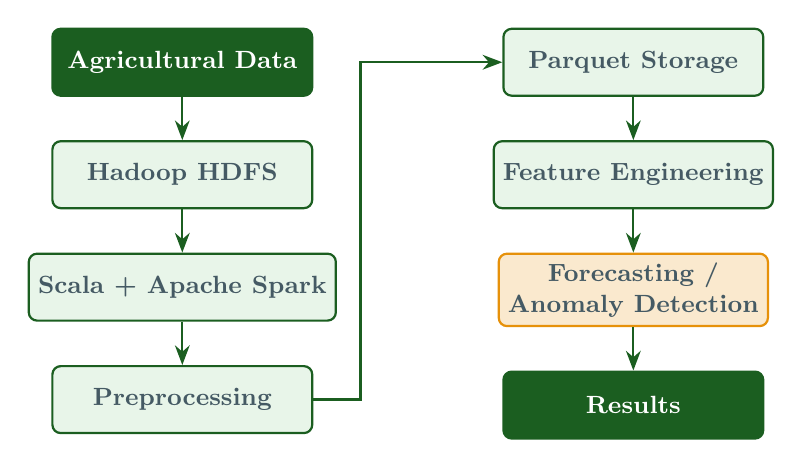
\begin{tikzpicture}[node distance=0.55cm]

    % ---- left column -------------------------------------------
    \node[hilitebox] (data)    {Agricultural Data};
    \node[flowbox, below=of data]    (hdfs)  {Hadoop HDFS};
    \node[flowbox, below=of hdfs]    (spark) {Scala + Apache Spark};
    \node[flowbox, below=of spark]   (prep)  {Preprocessing};

    \draw[arrowline] (data)  -- (hdfs);
    \draw[arrowline] (hdfs)  -- (spark);
    \draw[arrowline] (spark) -- (prep);

    % ---- right column ------------------------------------------
    \node[flowbox, right=2.4cm of data]  (parquet) {Parquet Storage};
    \node[flowbox, below=of parquet]     (feat)    {Feature Engineering};
    \node[ambox,   below=of feat]        (model)   {Forecasting /\\ Anomaly Detection};
    \node[hilitebox, below=of model]     (res)     {Results};

    \draw[arrowline] (parquet) -- (feat);
    \draw[arrowline] (feat)    -- (model);
    \draw[arrowline] (model)   -- (res);

    % ---- connector from left column to right column ------------
    \draw[arrowline] (prep.east) -- ++(0.6,0) |- (parquet.west);

  \end{tikzpicture}
  \end{center}
\end{frame}

%================================================================
% 7. DATA PREPROCESSING
%================================================================
\begin{frame}{Data Preprocessing}
  \vspace{0.25cm}
  All preprocessing is written in \textbf{Scala + Apache Spark}.

  \vspace{0.35cm}
  \begin{enumerate}\bigskipitems
    \item \textbf{Schema normalization} --- both datasets mapped to one common format.
    \item \textbf{Date parsing} --- different date formats converted safely.
    \item \textbf{Data quality classification} --- each record marked
          \textsc{valid} or defective.
    \item \textbf{Duplicate removal} --- repeated market reports removed.
    \item \textbf{Price outlier detection} --- unusual prices flagged per commodity.
    \item \textbf{Parquet conversion} and \textbf{year-based partitioning}.
  \end{enumerate}
\end{frame}

%================================================================
% 8. HADOOP HDFS STORAGE
%================================================================
\begin{frame}{Hadoop HDFS Storage}
  \vspace{0.1cm}
  \begin{columns}[T,onlytextwidth]
    \begin{column}{0.44\textwidth}
      \vspace{0.2cm}
      \begin{itemize}
        \setlength{\itemsep}{0.6em}
        \item[] \textbf{\textcolor{agriGreen}{NameNode}}\\
              {\small manages metadata}
        \item[] \textbf{\textcolor{agriGreen}{DataNodes}}\\
              {\small store actual data blocks}
        \item[] \textbf{\textcolor{agriAmber}{Replication = 3}}\\
              {\small each block has 3 copies}
        \item[] \textbf{\textcolor{agriAmber}{Block size = 128 MB}}\\
              {\small files split into 128 MB blocks}
      \end{itemize}
    \end{column}

    \begin{column}{0.54\textwidth}
      \begin{center}
      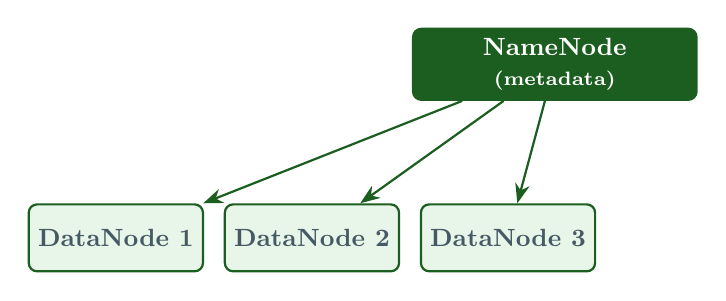
\begin{tikzpicture}[node distance=0.5cm]
        \node[hilitebox, minimum width=3.6cm] (nn) {NameNode\\ {\scriptsize(metadata)}};

        \node[flowbox, minimum width=1.7cm, below left=1.3cm and 0.15cm of nn] (dn2) {DataNode 2};
        \node[flowbox, minimum width=1.7cm, left=0.25cm of dn2]  (dn1) {DataNode 1};
        \node[flowbox, minimum width=1.7cm, right=0.25cm of dn2] (dn3) {DataNode 3};

        \draw[arrowline] (nn) -- (dn1);
        \draw[arrowline] (nn) -- (dn2);
        \draw[arrowline] (nn) -- (dn3);
      \end{tikzpicture}
      \end{center}

      \vspace{0.3cm}
      \begin{center}
        {\small Docker cluster:\\
        \textbf{1 NameNode + 3 DataNodes}}
      \end{center}
    \end{column}
  \end{columns}
\end{frame}

%================================================================
% 9. SYNTHETIC DATA SCALING
%================================================================
\begin{frame}{Synthetic Data Scaling}
  \vspace{0.2cm}
  To test scalability, we generated an \textbf{additional synthetic workload}.

  \vspace{0.4cm}
  \begin{center}
    \setlength{\tabcolsep}{12pt}
    \renewcommand{\arraystretch}{1.4}
    \begin{tabular}{lr}
      \toprule
      Real agricultural data      & $\approx$ 10.9 GB \\
      Synthetic scaled data       & $\approx$ 7.1 GB \\
      \midrule
      \textbf{Total experimental workload} & $\approx$ \textbf{18 GB} \\
      \bottomrule
    \end{tabular}
  \end{center}

  \vspace{0.45cm}
  \begin{itemize}
    \setlength{\itemsep}{0.5em}
    \item Generated from the \textbf{statistical patterns} of the real data
          (prices, commodities, markets, seasons).
    \item Every synthetic row is marked \texttt{data\_source = "synthetic\_scaled"}.
  \end{itemize}

  \vspace{0.25cm}
  \begin{block}{Important}
    \large Synthetic data is \textbf{NOT} presented as real government data.
    It is used \textbf{only} for scalability testing.
  \end{block}
\end{frame}

%================================================================
% 10. SCALA + APACHE SPARK
%================================================================
\begin{frame}{Scala + Apache Spark}
  \vspace{0.3cm}
  \begin{itemize}\bigskipitems
    \item \textbf{Scala} is the native language of Apache Spark.
    \item Spark splits data into \textbf{partitions} and processes
          them \textbf{in parallel}.
    \item \textbf{Spark SQL and DataFrames} used for cleaning and
          aggregation.
    \item \textbf{Window functions} used for duplicate removal and
          rolling price statistics.
    \item \textbf{Spark MLlib} is used for forecasting and anomaly
          modelling.
  \end{itemize}

  \vspace{0.35cm}
  \begin{center}
    {\large Entire preprocessing pipeline written in \textbf{Scala} ---
    no Pandas, no single-machine processing.}
  \end{center}
\end{frame}

%================================================================
% 11. REAL-TIME PROCESSING WITH KAFKA
%================================================================
\begin{frame}{Real-Time Processing with Kafka}
  \vspace{0.3cm}
  \begin{center}
  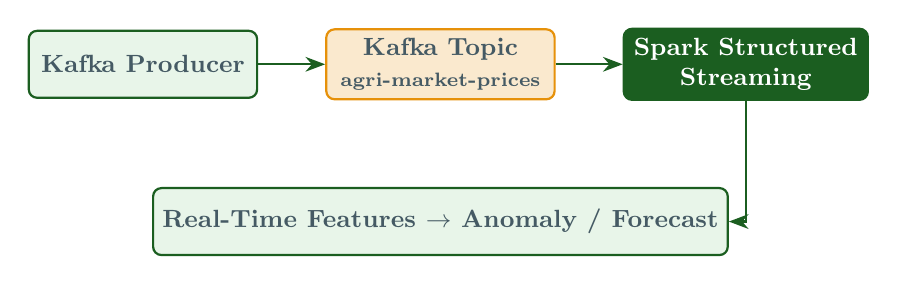
\begin{tikzpicture}[node distance=0.85cm]
    \node[flowbox, minimum width=2.9cm] (prod) {Kafka Producer};
    \node[ambox, minimum width=2.9cm, right=of prod] (topic)
        {Kafka Topic\\ {\scriptsize agri-market-prices}};
    \node[hilitebox, minimum width=3.1cm, right=of topic] (spark)
        {Spark Structured\\ Streaming};

    \draw[arrowline] (prod)  -- (topic);
    \draw[arrowline] (topic) -- (spark);

    \node[flowbox, minimum width=7.0cm, below=1.1cm of topic] (out)
        {Real-Time Features $\rightarrow$ Anomaly / Forecast};
    \draw[arrowline] (spark.south) |- (out.east);
  \end{tikzpicture}
  \end{center}

  \vspace{0.35cm}
  \begin{itemize}
    \setlength{\itemsep}{0.5em}
    \item Kafka \textbf{transports} market events; it is not a database.
    \item Historical records are \textbf{replayed} to simulate a live market feed.
    \item Spark Structured Streaming \textbf{consumes} and analyses them.
  \end{itemize}
\end{frame}

%================================================================
% 12. RESULTS
%================================================================
\begin{frame}{Results}
  \vspace{0.4cm}
  \begin{center}
    \setlength{\tabcolsep}{14pt}
    \renewcommand{\arraystretch}{1.45}
    \begin{tabular}{lr}
      \toprule
      \textbf{Metric} & \textbf{Value} \\
      \midrule
      Real records processed   & 132.9 million \\
      Duplicates removed       & 535,261 \\
      Records written          & 132.3 million \\
      Parquet size             & $\approx$ 1.2 GB \\
      Synthetic workload       & $\approx$ 7.1 GB \\
      \textbf{Total workload}  & $\approx$ \textbf{18 GB} \\
      \bottomrule
    \end{tabular}
  \end{center}

  \vspace{0.5cm}
  \begin{center}
    \large Storing data as \textbf{Parquet} reduced
    10.9 GB of CSV to about \textbf{1.2 GB}.
  \end{center}
\end{frame}

%================================================================
% 13. TECHNOLOGIES USED
%================================================================
\begin{frame}{Technologies Used}
  \vspace{0.3cm}
  \begin{center}
    \setlength{\tabcolsep}{14pt}
    \renewcommand{\arraystretch}{1.4}
    \begin{tabular}{ll}
      \toprule
      \textbf{Technology} & \textbf{Purpose} \\
      \midrule
      Hadoop HDFS            & Distributed storage \\
      Apache Spark           & Distributed processing \\
      Scala                  & Implementation language \\
      Spark SQL / DataFrames & Cleaning and aggregation \\
      Spark Structured Streaming & Real-time processing \\
      Apache Kafka           & Event streaming \\
      Spark MLlib            & Forecasting and anomaly models \\
      Parquet                & Compressed columnar storage \\
      Docker                 & HDFS cluster setup \\
      \bottomrule
    \end{tabular}
  \end{center}
\end{frame}

%================================================================
% 14. CONCLUSION
%================================================================
\begin{frame}{Conclusion}
  \vspace{0.4cm}
  \begin{itemize}\bigskipitems
    \item Successfully processed \textbf{132.9 million} real agricultural records.
    \item Built a complete \textbf{Scala + Spark} preprocessing pipeline.
    \item Stored data in \textbf{HDFS} with replication factor 3.
    \item Scaled the workload to $\approx$ \textbf{18 GB} using clearly
          marked synthetic data.
    \item Demonstrated \textbf{real-time streaming} using Kafka and Spark.
  \end{itemize}

  \vspace{0.4cm}
  \begin{center}
    \large The project shows how \textbf{Big Data tools} solve problems
    that traditional tools cannot handle.
  \end{center}
\end{frame}

%================================================================
% 15. FUTURE SCOPE
%================================================================
\begin{frame}{Future Scope}
  \vspace{0.4cm}
  \begin{itemize}\bigskipitems
    \item Deploy on a \textbf{real multi-node cluster} instead of a single machine.
    \item Connect to a \textbf{live government market feed} instead of replay.
    \item Improve forecasting accuracy using \textbf{advanced ML models}.
    \item Build an \textbf{interactive dashboard} for farmers and officials.
    \item Add \textbf{alerts} when abnormal price behaviour is detected.
  \end{itemize}
\end{frame}

%================================================================
% THANK YOU
%================================================================
\begin{frame}[plain]
  \vspace{1.6cm}
  \begin{center}
    {\color{agriGreen}\Huge\bfseries Thank You}

    \vspace{0.8cm}
    
\begin{tikzpicture}
      \draw[agriAmber, line width=1.2pt] (0,0) -- (5,0);
    \end{tikzpicture}

    \vspace{0.8cm}
    {\color{agriGrey}\Large Questions?}
  \end{center}
\end{frame}

\end{document}
